\chapter*{Kivonat}

A szakdolgozatban fűtési rendszerek modell-prediktív szabályzásának lehetőségeit vizsgálom Matlab Simulinkben.
Végighaladok az MPC tervezés lépésein, a tervezést és a validálást is szimulált szakaszmodellen végzem. A szakaszmodellt egy helyiség és annak fűtési rendszere alkotja, a fűtés hője a helyiségből külső homlokzaton távozik a környezet felé. Az állandósult állapotban szükséges fűtési teljesítményt képlettel számítom, ebből kapható a beavatkozó jel egy adott teljesítményigényhez. A hőkapacitásokat és hőátadási, hővezetési tényezőket Simscape modell tartalmazza%(\ref{table_heater_parameters}. és \ref{table_house_parameters}. táblázat)
, meghatározva a szakasz dinamikáját. Megvizsgálom az MPC predikciós horizontjának, költségfüggvényének illetve mintavételi idejének hatását a zárt szabályzási kör viselkedésére. 

%tranziens viselkedését
%A szimulációhoz felállított modellhez számításokra is szükség van,
%Állandósult állapotra felírt képlet adja a szükséges fűtési teljesítményt

A tervezési lépéseket ezután valós, fizikai modellen is elvégzem, így látható lesz, hogy egy kész házra, vagy annak egy részére mennyi munkával jár a szabályzó beállítása. Ha a modellezésre, hangolásra fordított idő megtérül, azaz komfortnövekedéssel, illetve az üzemeltetési költségek csökkenésével jár, akkor az iContrALL intelligens otthon rendszerbe is beilleszthetők lesznek az új funkciók.


\chapter{Bevezetés}
Az Európai Unió energiafogyasztásának 40\%-át az épületek adják, a szén-dioxid-kibocsátás 36\%-áért felelősek. Az energiahatékonyság növelése kiemelten fontos: a korszerűbb közintézmények, munkahelyek, lakóingatlanok olcsóbban fenntarthatók és alacsonyabb károsanyag-kibocsátás mellett az emberek életminőségét is javítják.

Az új épületekre egyre szigorodó követelmények vonatkoznak\footnote{2021-ben használatba vett ingatlanoknak már teljesíteniük kell a közel nulla energiaigényű épületekre \cite{NZEB} vonatkozó szabályokat. }.
A törvények előírják energetikai tanúsítvány készítését szerte az Unióban, ami ellenőrzi az épület megfelelőségét energetikai szempontból.
Azok a legújabb építésű, fenntartható irodaházak, amelyek LEED, illetve WELL minősítést kapnak, az emberek egészségének és jó közérzetének fenntartását is segítik\footnote{A LEED egy komplex minősítési rendszer, a szakdolgozat tematikájához az \textit{Energia és légkör} kategóriája tartozik leginkább. Bővebben: https://www.terc.hu/tudastar/leed \\
A WELL hét szempont alapján értékel - víz, egészséges táplálkozás, természetes fény, testmozgás, kényelem és szellemi frissesség ‒ és ezek technikai feltételeire tesz javaslatokat.}.

Ilyen fejlett technológiákat felvonultató épületekben nagy szerepet játszanak az épületgépészeti rendszerek\footnote{Épületgépészeti rendszer a \cite{TNM2006} rendelet szerint a  HVAC (heating, ventilation, and air conditioning), a melegvíz-ellátásra és világításra szolgáló berendezések összessége.},
a 7/2006. TNM rendelet \cite{TNM2006} is megfogalmaz szabályokat és ajánlásokat ezzel kapcsolatban. Eszerint \say{új fűtési rendszer létesítésekor és meglévő fűtési rendszer korszerűsítésekor a helyiségenkénti hőmérséklet-szabályozást javasolt megvalósítani gazdaságossági számítás\footnote{A gazdaságossági számítás egy teljes élettartamra vonatkozó minimumköltséget céloz meg.} alapján}.
	
	%    Ezekhez tartozó költségoptimalizált szint: az energiahatékonyság azon szintje, amely egy épület, vagy valamely az épületek energetikai jellemzőinek meghatározásáról szóló rendeletben meghatározott épületelem becsült gazdasági élettartama folyamán a legalacsonyabb költséget eredményezi.
	% https://ec.europa.eu/energy/en/content/eu-countries-2018-cost-optimal-reports}}. 

	% Számos megtakarítási forma már régóta él a köztudatban, például a szigetelés, az ablakcsere. Alacsonyabb besorolás esetén az energetikai tanúsítványban is szerepel javaslat a korszerűsítésre. %Az ágazat úttörői az építészek, többnyire a szerkezetek tervezésénél veszik figyelembe a fenti szempontokat.
	%Az üzemeltetési időszakra viszont kevesebb figyelem kerül, szerencsére manapság már a teljes élettartamra vetített költséget is figyelembe szokás venni.

	%Sokszor ilyen esetben csak az épületszerkezetek kialakítására fordítanak kellő figyelmet - az előírások is erre vonatkoznak, az épületgépészeti rendszerek automatizálása viszont kevésbé elterjedt.

Munkámban szeretnék megvalósítani egy helyiségenkénti hőmérséklet-szabályozást, ezen keresztül pedig megmutatni a különböző fűtési típusok viselkedését egy helyiségen belül.



%\section{A modell felírásához tartozó megállapítások}

%\paragraph{A szabályzó:}

 

% a szabályzót ezután egy fizikai rendszerre is megtervezem, hogy azt laborkörülmények közt kipróbáljam. A szabályzás beavatkozó jelei a szelepek, amellyel a fűtési teljesítmény befolyásolható, a visszacsatolás belső hőmérséklet mérésével adódik.

\section*{A modell típusa, hatóköre}

A szabályozáshoz a klasszikus elképzelések szerint ismerjük a szabályzott szakasz viselkedését, ellenkező esetben identifikálnunk kell azt. Ismert hálózatokra felírható gerjesztés-válasz kapcsolat, például átviteli függvények formájában. % Viszont akkor is érdemes lehet identifikálni, ha analitikusan túl hosszadalmas volna az átviteli függvény felírása.
%Épületfizikai összefüggéseket felhasználva egyenleteket is fel lehet írni a hőfelvételre, hőleadásra. Ezen összefüggésekkel egyenértékű átviteli függvény is felírható, ha a rendszer bemeneteire gerjesztéseket adunk és mérjük a kimeneteket.  %\cite{AFRAM2014343}

A szabályozott szakasz először egy szimulált hálózat\footnote{A szimulációban sokkal könnyebben megfigyelhető az egyes paraméterek hatása, így lépésről lépésre megérthető a rendszer viselkedése.}, emiatt fizikai modell felírása mellett döntöttem. A \textit{\ref{chap:helyiseg}-\ref{chap:futotest}. fejezetekben} felállítom egy helyiség és a hozzátartozó fűtőtestek modelljét. %A modellalkotást méretezési szabályok is befolyásolják. Publikációk, könyvek, adatlapok alapján validálom a felírt összefüggéseket, az ottani mérések adataiból kiindulva. 

%(TOVBÁBBI fűtőtestek mérése a \cite[313, 361.~o.]{Herz})

%A belső hőmérsékletet számos jellemző befolyásolhatja. 
A szabályzás a helyiség hőveszteségét egyenlíti ki, amit az alacsonyabb külső hőmérséklet ($t_e$) okoz. A külső falon és az ablakon hő távozik, amelyet radiátoros és padlófűtéssel egyenlíthetünk ki.

%A szabályozás helyiségekre van bontva, a modellben is csak egy helyiség és annak fűtési rendszere szerepel. %Ezen a szinten 
%
%A 2.1 fejezetet kellene itt bevezetni.
%
%
%\footnote{A referenciajelbe az időjárás-előrejelzési adatok is beleszólhatnak a energiamegtakarítás érdekében.}.
%
\begin{figure}[h]
	\centering
	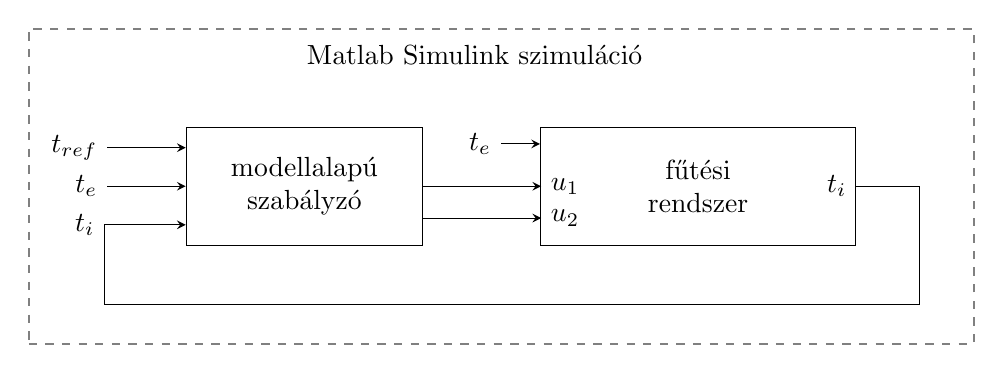
\begin{tikzpicture}[>=stealth,
	outer/.style={draw=gray,dashed,thick,inner sep=5pt}]
	
	% nagy blokkok
	\node[draw,rectangle, minimum height=1.5cm,minimum width=4cm] (plant) at (5,2.5) {\parbox{2cm}{\centering fűtési\\rendszer}};
	\node[draw,rectangle, minimum height=1.5cm,minimum width=3cm] (Control) at (0,2.5) {\parbox{2.5cm}{\centering modellalapú\\szabályzó}};
	
	% szaggatott vonal
	\node[draw,outer,rectangle, minimum height=4cm,minimum width=12cm,
	label={[label distance=-0.1cm, anchor=north]100:Matlab Simulink szimuláció}] (keret) at (2.5,2.5) {};
	
	
	% plant bemenetei
	\draw [->] (Control.0) node[right]{} -- +(15mm,0) node[right]{${u_{1}}$};
	\draw [->] (Control.345) node[right]{} -- +(15mm,0) node[right]{${u_{2}}$};
	\draw [<-] (plant.165) node[right]{} -- +(-5mm,0) node[left]{${t_{e}}$};
	%\draw [<-] (plant.90) node[right]{} -- +(0,3mm) node[right]{$t_{e}$};
	%\draw [<-] (plant.162) node[right]{} -- +(-10mm,0) node[left]{$t_{ref}$};
	
	% szabályzó bemenetei
	% a -| és |- máshogy fog törni, ha unconstraintelt.
	\draw [->] (plant.0)  node[left]{$t_i$} -|++(0.8,-1.5) -| ++(-9.25,0) |-  ++(-1.1,0) |- node[left]{$t_i$} (Control.198);
	
	\draw [<-] (Control.180) node[right]{} -- +(-10mm,0) node[left]{$t_{e}$};
	\draw [<-] (Control.162) node[right]{} -- +(-10mm,0) node[left]{$t_{ref}$};
	\end{tikzpicture}
	\caption{A szimuláció felépítése}
	\label{tikz:simulation-basic}
\end{figure}

%
\section*{A szabályozás folyamata, szabályzótervezés}
A szabályzó a  modell alapján olyan szelepekkel képes beavatkozni, melyekkel a fűtőtestbe beáramló vízmennyiség korlátozható. A szelepek ($u_1, u_2$) állását folytonosan tudom változtatni. A modell bemenetei a szelepek állásai és a külső hőmérséklet, kimenete a belső hőmérséklet ($t_i$).  A belső és külső hőmérsékletet mérem, ez alapján történik a szabályzás. 
%
A tervezés lépései a \textit{\ref{chap:ident}-\ref{chap:control}. fejezetben} olvashatóak.
%Az alapértelmezett paramétereket módosítom a fizikai korlátoknak megfelelően,  amelyek a beavatkozókra vagy a szakaszra vonatkoznak.
%
%Az MPC-nek rendkívül sok paraméterezési lehetősége van, amitől függően a szabályzás agresszívebb vagy robusztusabb lehet.   %---- (kazánok \cite[235.~o.]{Herz} szerint: kazánok hatásfoka, túlméretezése. )
%Az MPC szabályozás gyakorlati kipróbálásához fizikai tesztrendszert állítunk fel, itt az MPC tervezési kérdésekre koncentrálok, átviteli függvény modellből.
%
%
\section*{Eredmények gyakorlati kipróbálása, további lehetőségek}
%
A szabályzótervezés lépéseit egy fizikai rendszerre is elvégzem, hogy további tapasztalatokat szerezzek. Végül áttekintem, hogy a szabályzás használatának milyen gyakorlati lehetőségei vannak, mind technikai értelemben, mind piacképesség szempontjából. Végül összefoglalom az elért eredményeket.


%, melynek paramétereit energetikai tanúsítványból vehetjük. Ezzel egy közelítő modelljét megkapjuk a háznak, terepi mérések nélkül is lehetséges a szabályzás. A telepítés ideje lecsökkenthető, hiszen a hosszas kalibrálás elmarad.  A modellezéshez külön írom fel a helyiség és a fűtőtestek modelljét.%Természetesen bevethetők zárt körben végzett identifikációs módszerek, adaptív szabályzók is.




%Ehhez először áttekintettem a hőátadás lehetséges formáit és forrásait.
%Ezután fűtőtestek modelljét állítom fel.




%\pagebreak

 %Arra jutottam, hogy ha a levegő hőmérsékletére szabályzok, akkor az abba beleszóló tényezőket veszem sorra:
%\begin{itemize}[noitemsep,topsep=0pt,parsep=0pt,partopsep=0pt]
%	\item konvektív hőátadás: a felszín közelében felmelegedett levegő áramlani kezd
%	\item radiatív hőátadás: sugárzással kibocsátott energia a környezetbe
%\end{itemize}

%\begin{figure}[h]
%	\centering
%	\includegraphics[width=8cm]{figures/konvrad}
%	\caption{Alacsony hőmérsékletű fűtés és magas hőmérsékletű hűtés c. könyv ábrája}
%		%\footnote{Jan Babiak, rehva Guidebook No.7}
%\end{figure}


%A levegő hőmérsékletére ezek a következőképp hatnak a leginkább:
%\begin{itemize}[noitemsep,topsep=0pt,parsep=0pt,partopsep=0pt]
%	\item a fűtőtestek konvektív és radiatív hőátadással is melegítik a környezetet
%	\item a radiatív energiát a tárgyak, falak nyelik el, amik ezáltal felmelegszenek (mintegy kapacitásként lesz egy hőtároló tömeg, ami a fűtés kikapcsolásával fenntartja a hőmérsékletet / lassítja a hűlést)
%	\item a fűtetlen falfelületek hűtik a szobát (külső hőmérséklet befolyása)
%\end{itemize}
%
%Így a kezdeti modellben azzal a feltételezéssel élek, hogy ezen kívül más hatás nem lép fel.
%
%A modellben feltételezem, hogy a fűtőtest felületi hőmérsékletével tudunk beavatkozni. A modellben paraméter a fűtőtestek hőátadási tényezője és felülete. Zavarásként (?) hat a külső hőmérséklet értéke, amit mérni is tudunk. Kimenet a belső hőmérséklet (térben konstansnak véve azt / átlagolva a szoba levegőjére)
%
%A modell felírásához a fűtőtest tulajdonságain kívül szükség van a szobában található levegő mennyiségére is. A zavarás hatását is fel kell írni, azaz hogy egy külső hőmérsékletváltozás hogyan jelenik meg a kimeneten. (Célszerű itt egy átviteli függvényt felírni először, szuperpozíciószerűen. A zavarás viszont nem a modell bemenetén és nem is a kimenetén hat.)

%A felírandó átviteli függvények:
%
%\begin{itemize}[noitemsep,topsep=0pt,parsep=0pt,partopsep=0pt]
%	\item levegő felmelegedése konstans külső hőmérsékletet feltételezve, fűtőtest egységugrással
%	\item levegő felmelegedése fűtés kikapcsolt állapota mellett, környezeti hőmérséklet ugrásával
%\end{itemize}
%
%Ezeket ráadtam a rendszerre és két bemenetű, egy kimenetű rendszerként identifikáltam.

%\pagebreak


%\subsubsection{Modellparaméterek}

%\subsection{-----}
%
%Fűtési típusok szerint:
%
%\begin{itemize}[noitemsep,topsep=0pt,parsep=0pt,partopsep=0pt]
%	\item radiátoros fűtés hőátvitele
%	\item padlófűtés hőátvitele
%\end{itemize}
%
%A fentiekre különböző értékű lesz a 
%
%\begin{itemize}[noitemsep,topsep=0pt,parsep=0pt,partopsep=0pt]
%	\item hőátadási tényező
%	\item hőtároló tömeg
%	\item költségfüggvény?
%	\item előremenő vízhőmérséklet és ezzel a leadott teljesítmény maximumértéke
%\end{itemize}
%
%ami így eltérő ház-modelleket fog eredményezni.


\pagebreak